%!TEX root = PaulAllen_Y362220X_MST125_TMA_02.tex
\documentclass{tufte-handout}


\usepackage{style}


\newenvironment{amatrix}[1]{%
  \left(\begin{array}{@{}*{#1}{c}|c@{}}
}{%
  \end{array}\right)
}

\newenvironment{longdiv}[1]{%
  \(\begin{array}{r@{}*{#1}{c} r r}
}{%
  \end{array}\)
}

\begin{document}
\bibliography{biblio.bib} 
\tma{02}

%question one

\begin{question}

\qpart
\qsubpart

\[ g(x,y) = (2x,7y) \]

\begin{align*}
    \begin{pmatrix}
        a & b \\
        c & d
    \end{pmatrix}
    \times
    \begin{pmatrix}
        x \\
        y
    \end{pmatrix}
    &=
    \begin{pmatrix}
        2x\\
        7y
    \end{pmatrix}\\[8pt]
    \begin{pmatrix}
        ax + by \\
        cx + dy
    \end{pmatrix}
    &=
    \begin{pmatrix}
        2x + 0y\\
        0x + 7y
    \end{pmatrix}\\[8pt]
    &=
    \begin{pmatrix}
        2 & 0 \\
        0 & 7
    \end{pmatrix}\\
\end{align*}

This is a diagonal scaling, scale by \( 2 \) in \( x‐ \)direction, \( 7 \) in \( y‐ \)direction.

\vspace{4cm}
\qsubpart

\[ h(x,y) = (x,4x+y) \]

\begin{align*}
    \begin{pmatrix}
        a & b \\
        c & d
    \end{pmatrix}
    \times
    \begin{pmatrix}
        x \\
        y
    \end{pmatrix}
    &=
    \begin{pmatrix}
        x + y\\
        4x + y
    \end{pmatrix}\\[8pt]
    \begin{pmatrix}
        ax + by \\
        cx + dy
    \end{pmatrix}
    &=
    \begin{pmatrix}
        x + 0y\\
        4x + y
    \end{pmatrix}\\[8pt]
    &=
    \begin{pmatrix}
        1 & 0\\
        4 & 1
    \end{pmatrix}\\
\end{align*}

This is a shear transformation.

\vspace{4cm}
\qsubpart

\[ k(x,y) = (y,x) \]

\begin{align*}
    \begin{pmatrix}
        a & b \\
        c & d
    \end{pmatrix}
    \times
    \begin{pmatrix}
        x \\
        y
    \end{pmatrix}
    &=
    \begin{pmatrix}
        y\\
        x
    \end{pmatrix}\\[8pt]
    \begin{pmatrix}
        ax + by \\
        cx + dy
    \end{pmatrix}
    &=
    \begin{pmatrix}
        0x + y\\
        x + 0y
    \end{pmatrix}\\[8pt]
    &=
    \begin{pmatrix}
        0 & 1\\
        1 & 0
    \end{pmatrix}\\
\end{align*}

This swaps \( x \) and \( y \).

\vspace{3cm}
\qpart

\[ g = \begin{pmatrix}
    2 & 0 \\
    0 & 7
    \end{pmatrix}
    \qquad
    h = \begin{pmatrix}
        1 & 0 \\
        4 & 1
    \end{pmatrix}
    \qquad
    k = \begin{pmatrix}
        0 & 1 \\
        1 & 0
    \end{pmatrix} 
\]

\[ f = k \circ h \circ g \]

\begin{align*}
    \stext{First we find \( h \circ g \) }\\
    &= h \circ g \\
    &= \begin{pmatrix}
        1 & 0 \\
        4 & 1
    \end{pmatrix}
    \times
    \begin{pmatrix}
        2 & 0 \\
        0 & 7
    \end{pmatrix}\\[8pt]
    &= \begin{pmatrix}
        1 \times 2 + 0 \times 0 & 1 \times 0 + 0 \times 7 \\
        4 \times 2 + 1 \times 0 & 4 \times 0 + 1 \times 7
    \end{pmatrix}\\
    &= \begin{pmatrix}
        2 & 0 \\
        8 & 7
    \end{pmatrix}\\
\stext{Now we find \( k \circ h \circ g \)}\\
    \mathbf{A}  &= k \circ \begin{pmatrix}
        2 & 0 \\
        8 & 7
    \end{pmatrix}\\[8pt]
    &= \begin{pmatrix}
        0 & 1 \\
        1 & 0
    \end{pmatrix}
    \times
    \begin{pmatrix}
        2 & 0 \\
        8 & 7
    \end{pmatrix}\\[8pt]
    &= \begin{pmatrix}
        0 \times 2 + 1 \times 8 & 0 \times 0 + 1 \times 7 \\
        1 \times 2 + 0 \times 8 & 1 \times 0 + 0 \times 7
    \end{pmatrix}\\[8pt]
    &= \begin{pmatrix}
        8 & 7 \\
        2 & 0
    \end{pmatrix}\\
    \snote{As required}
\end{align*}

\vspace{3cm}
\qpart

\marginnote{To find the determiate of a matrix, we can use the formula:\[ Det A = ad - bc \]}
\marginnote{To find the inverse of a matrix we use \[ \mathbf{A^{-1}} = \frac{1}{Det A}\begin{pmatrix}
        d & -b \\
        -c & a
    \end{pmatrix} \]}


First we have to find the determinant of \( f \).

\begin{align*}
    Det A &= Det \begin{pmatrix}
        8 & 7 \\
        2 & 0
    \end{pmatrix}\\[8pt]
    &= 8 \times 0 - 7 \times 2\\
    &= -14
\end{align*}

As \( Det A \neq 0 \) \( f \) is invertable 

\begin{align*}
    \stext{Hence the matrix that represents \( f^{-1} \) is}
    f^{-1} &= \frac{1}{Det A} \times \begin{pmatrix}
        0 & -7 \\
        -2 & 8
    \end{pmatrix}\\[8pt]
    &= \frac{-1}{14} \times \begin{pmatrix}
        0 & -7 \\
        -2 & 8
    \end{pmatrix}\\[8pt]
    &= \frac{1}{14} \times \begin{pmatrix}
        0 & 7 \\
        2 & -8
    \end{pmatrix}\\[8pt]
    &= \begin{pmatrix}
        0 & \frac{1}{2} \\
        \frac{1}{7} & -\frac{4}{7}
    \end{pmatrix}\\
\end{align*}

\vspace{3cm}
\qpart

First to find the coordinates of the point in the domain of \( f \) 
that is mapped to a general point \( (x,y) \) in the codomain of \( f \).

\begin{align*}
    \stext{Each point \( (x,y) \) is the image under \( f \) of the point
    \( f^{-1}(x,y) \) }
    \mathbf{A^{-1}}\begin{pmatrix}
        x \\
        y
    \end{pmatrix}
    &= \begin{pmatrix}
        0 & \frac{1}{2} \\
        \frac{1}{7} & -\frac{4}{7}      
    \end{pmatrix}
    \times
    \begin{pmatrix}
        x \\
        y
    \end{pmatrix}\\[8pt]
    &= \begin{pmatrix}
        0 \times x + \frac{1}{2} \times y \\
        \frac{1}{7} \times x - \frac{4}{7} \times y
    \end{pmatrix}\\[8pt]
\stext{Hence  \( f \) maps the point \( (\frac{y}{2}, \frac{x - 4y}{7}) \)
to the point \( (x,y) \) }
\end{align*}

\marginnote{The general equation of the unit circle is \[ x^{2} + y^{2} = 1 \]}

\begin{align*}
\stext{Substitute these values into the unit circle to find the equation of the image \( f(C) \)}\\[8pt]
    (\frac{y}{2}^{2} + \frac{x - 4y}{7}^{2}) &= 1\\[8pt]
\stext{Mulitplying out the brackets}\\[8pt]
    \frac{y^{2}}{4} + \frac{x^{2} - 8xy + 16y^{2}}{49} &= 1\\[8pt]
\stext{Multiplying through by \( 196 \)}\\[8pt]
    49y^{2} + 4x^{2} - 32xy + 64y^{2} &= 196\\[8pt]
\stext{Combining like terms, leaves us with the equation of \( f(C) \)}
    \frac{1}{196}(4x^{2} - 32xy + 113y^{2}) &= 1\\[8pt]
\stext{Putting this into the form \( ax^{2} + bxy + cy^{2} = d \)}
    4x^{2} - 32xy + 113y^{2} &= 196\\[8pt]
\stext{This is the equation of the image \( f(C) \)}
\stext{where \( a = 4, b = -32, c = 113, d = 196 \)}
\end{align*}

\vspace{3cm}
\qpart

The area of the unit circle is \( \pi \) the area of \( f(C) \) is given by the fact
that linear transformations scale the area by the absolute value of the determinant of 
the transformation matrix.

\begin{align*}
    \stext{The area of the image \( f(C) \) is}
    Area(f(C)) &= \vert Det f \vert \times Area(C)\\[8pt]
    &= 14 \times \pi\\
    &= 14\pi   
\end{align*}

\end{question}

\clearpage

%question two
\begin{question}

    \qpart
    \qsubpart

 The affine transformation \( f \) that maps the points \( (0,0), (1,0), (0,1) \) to the points
    \( (-3,4), (-2,4), (-3,5) \) can be represented by the matrix equation   

\[ f(x) = \mathbf{A}x + \mathbf{a} \]

\begin{align*}
    \stext{Let, \( \mathbf{a}, \mathbf{b}, \mathbf{c} \) be the new vector positions. }
    \mathbf{A}=
    \begin{pmatrix}
        \mathbf{b}x-\mathbf{a}x & \mathbf{c}x-\mathbf{a}x \\
        \mathbf{b}y-\mathbf{a}y & \mathbf{c}y-\mathbf{a}y
    \end{pmatrix} 
    \stext{and} 
    \mathbf{a} = 
    \begin{pmatrix}
        \mathbf{a}x \\
        \mathbf{a}y
    \end{pmatrix}\\[8pt]
    \stext{We can set up the matrices for the transformation}\\[8pt]
    \begin{pmatrix}
        -2-(-3) & -3-(-3) \\
        4-4 & 5-4
    \end{pmatrix}
    &=
    \begin{pmatrix}
        1 & 0 \\
        0 & 1
    \end{pmatrix}
\stext{Hence}
f(x) &=
    \begin{pmatrix}
        1 & 0\\
        0 & 1
    \end{pmatrix}x
    +
    \begin{pmatrix}
        -3\\
        4
    \end{pmatrix}
\end{align*}

\vspace{3cm}

\qsubpart

As the matrix is the identity matrix \((f)\) is a translation and hence 
has no fixed points.

    \qpart
    \begin{align*}
        \stext{The matrix to represent reflection in the line \( y = -x \) is}
        R &= \begin{pmatrix}
            0 & -1\\
            -1 & 0
        \end{pmatrix}\\[8pt]
        \stext{To reflect in the line \( y = -x + 7 \), use translation \( h \) to the origin, apply \( R \), then translate back with \( h^{-1} \)}\\[8pt]
        \stext{Let \( h(x, y) = (x, y - 7) \), \( h^{-1}(x, y) = (x, y + 7) \)}\\[8pt]
        \stext{Apply the composite transformation \( f(x) = h^{-1}(R(h(x))) \)}\\[8pt]
        \stext{Step 1: Translate down by 7}
        h(x) &= \begin{pmatrix} x \\ y - 7 \end{pmatrix}\\[8pt]
        \stext{Step 2: Reflect in \( y = -x \)}
        R \times h(x) &= \begin{pmatrix}
            0 & -1 \\
            -1 & 0
        \end{pmatrix}
        \times
        \begin{pmatrix}
            x \\
            y - 7
        \end{pmatrix}
        =
        \begin{pmatrix}
            -(y - 7) \\
            -x
        \end{pmatrix}
        =
        \begin{pmatrix}
            7 - y \\
            -x
        \end{pmatrix}\\[8pt]
        \stext{Step 3: Translate up by 7}
        f(x) &= h^{-1}(R(h(x))) =
        \begin{pmatrix}
            7 - y \\
            -x + 7
        \end{pmatrix}\\[8pt]
        \stext{Therefore, the matrix form is:}
        B &= \begin{pmatrix}
            0 & -1 \\
            -1 & 0
        \end{pmatrix}, \quad
        b = \begin{pmatrix}
            7 \\
            7
        \end{pmatrix}
    \end{align*}

\end{question}

\clearpage
%question three

\begin{question}

\qpart

\[ \frac{5x^{3} - 11x^{2} - 99x - 72}{x^{2} - 3x - 18} \]

First we need to divide the polynomials using long division.

\polylongdiv{5x^{3}-11x^{2}-99x-72}{x^{2}-3x-18}

\begin{align*}
    \frac{5x^{3} - 11x^{2} - 99x - 72}{x^{2} - 3x - 18} &= 5x + 4 + \frac{3x}{x^{2} - 3x - 18}\\[8pt]
\stext{using partial fractions on the remainder}\\[8pt]
    \frac{3x}{x^{2} - 3x - 18} &= \frac{A}{x - 6} + \frac{B}{x + 3}\\[8pt]
\stext{Using augmented matrix to solve for \( A \) and \( B \)}\\[8pt]
    3x &= A(x + 3) + B(x - 6)\\[8pt]
    &= Ax + 3A + Bx - 6B\\[8pt]
    &= (A + B)x + (3A - 6B)\\[8pt]
\stext{Setting up the augmented matrix}\\[8pt]
    \begin{amatrix}{2}
        3 & -6 & 0\\
        1 & 1 & 3
    \end{amatrix}\\[8pt]
\snote{Subtract 3 times R2 from R1}\\[8pt]
    \begin{amatrix}{2}
        0 & -9 & -9\\
        1 & 1 & 3
    \end{amatrix}\\[8pt]
\snote{Divide R1 by -9}\\[8pt]
    \begin{amatrix}{2}
        0 & 1 & 1\\
        1 & 1 & 3
    \end{amatrix}\\[8pt]
\snote{Subtract R1 from R2}\\[8pt]
    \begin{amatrix}{2}
        0 & 1 & 1\\
        1 & 0 & 2
    \end{amatrix}\\[8pt]
\stext{Hence we can write}\\[8pt]
    \frac{3x}{x^{2} - 3x - 18} &= \frac{2}{x - 6} + \frac{1}{x + 3}\\[8pt]
\stext{Giving us the full expression}\\[8pt]
    \frac{5x^{3} - 11x^{2} - 99x - 72}{x^{2} - 3x - 18} &= 5x + 4 + \frac{2}{x - 6} + \frac{1}{x + 3}\\[8pt]
\end{align*}

\qpart
\subsection*{Question 3 (b)}
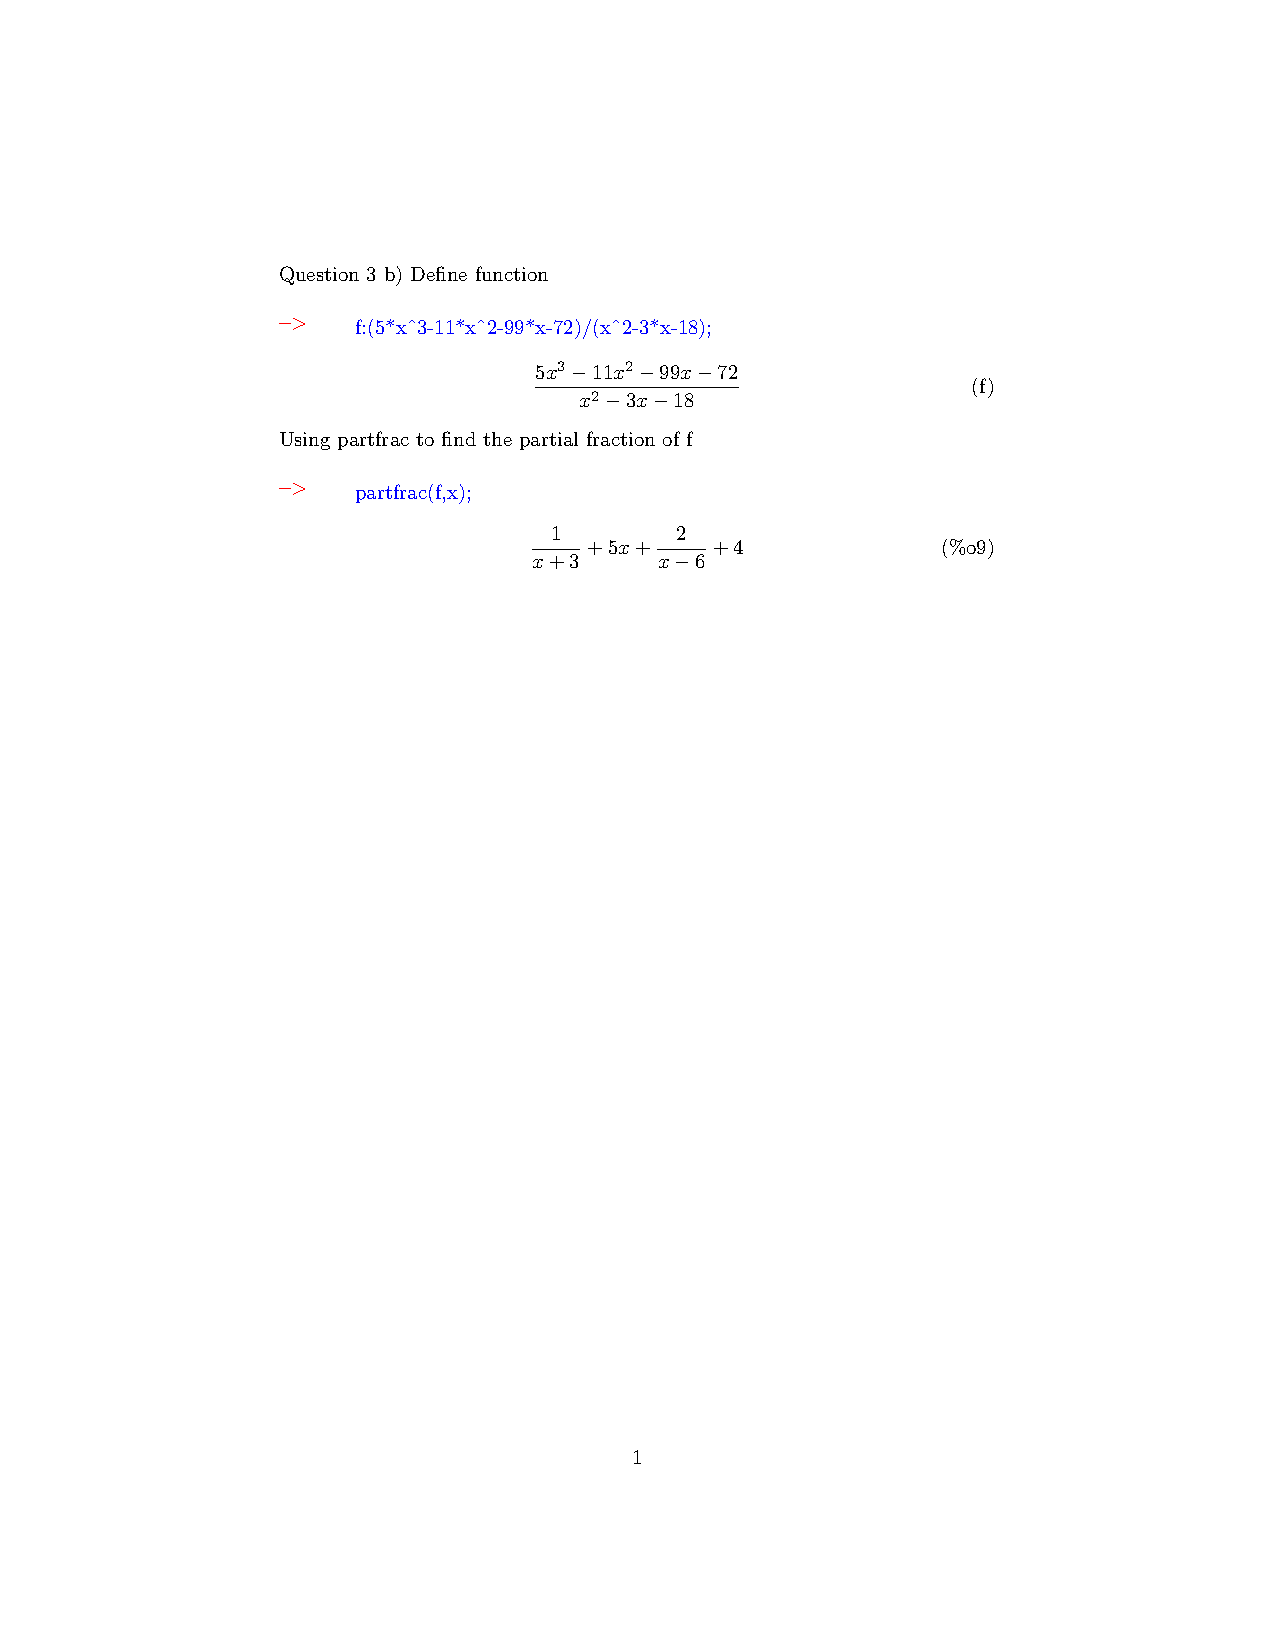
\includepdf[pages=-]{question_3_b.pdf}
\clearpage

\qpart

\begin{align*}
\int \frac{5x^{3} - 11x^{2} - 99x - 72}{x^{2} - 3x - 18} \dd{x} &= \int \left(5x + 4 + \frac{2}{x - 6} + \frac{1}{x + 3}\right) \dd{x}\\[8pt]
&= \int 5x \dd{x} + \int 4 \dd{x} + \int \frac{2}{x - 6} \dd{x} + \int \frac{1}{x + 3} \dd{x}\\[8pt]
&= \frac{5}{2}x^{2} + 4x + 2\ln|x - 6| + \ln|x + 3| + C\\[8pt]
&= \frac{5}{2}x^{2} + 4x + 2\ln(x - 6) + \ln(x + 3) + C
\end{align*}

\end{question}

\clearpage
%question four

\begin{question}

    \[ f(x) = \frac{2 - x}{x^{2} + 21} \]

\qpart

The domain of \( f \) is all real numbers \( \mathbb{R} \), since the denominator \( x^{2} + 21 \) is never zero.

For the intercepts;

\begin{align*}
\stext{To find the \( x \)-intercept, set \( f(x) = 0 \)}\\
    0 &= \frac{2 - x}{x^{2} + 21}\\
    2 - x &= 0\\
    x &= 2\\
\stext{So the \( x \)-intercept is at } (2, 0)\\[8pt]
\stext{To find the \( y \)-intercept, set \( x = 0 \)}\\
    f(0) &= \frac{2 - 0}{0^{2} + 21}\\
    &= \frac{2}{21}\\
    \stext{So the \( y \)-intercept is at } (0, \frac{2}{21})
\end{align*}

\vspace{3cm}

\qpart

For the stationary points, we need to find the derivative of \( f \) and set it to zero.

\begin{align*}
    f(x) &= \frac{2 - x}{x^{2} + 21}\\[8pt]
\stext{Using the quotient rule, where \( u = 2 - x \) and \( v = x^{2} + 21 \)}\\[8pt]
    f'(x) &= \frac{(v \times u' - u \times v')}{v^{2}}\\[8pt]
    &= \frac{((x^{2} + 21)(-1) - (2 - x)(2x))}{(x^{2} + 21)^{2}}\\[8pt]
    &= \frac{-x^{2} - 21 - (4x - 2x^{2})}{(x^{2} + 21)^{2}}\\[8pt]
    &= \frac{-x^{2} - 21 - 4x + 2x^{2}}{(x^{2} + 21)^{2}}\\[8pt]
    &= \frac{x^{2} - 4x - 21}{(x^{2} + 21)^{2}}
\stext{Setting the numerator to zero for stationary points}\\[8pt]
    x^{2} - 4x - 21 &= 0\\[8pt]
    (x + 3)(x - 7)  &= 0\\[8pt]
    x &= -3 \quad \text{or} \quad x = 7\\
\stext{So the stationary points are at } (-3, f(-3)) \text{ and } (7, f(7))\\[8pt]
\stext{Calculating \( f(-3) \)}\\[8pt]
    f(-3) &= \frac{2 - (-3)}{(-3)^{2} + 21}\\
    &= \frac{5}{9 + 21}\\
    &= \frac{5}{30}\\
    &= \frac{1}{6}\\
\stext{So the stationary point is at } (-3, \frac{1}{6})\\[8pt]
\stext{Calculating \( f(7) \)}\\[8pt]
    f(7) &= \frac{2 - 7}{7^{2} + 21}\\
    &= \frac{-5}{49 + 21}\\ 
    &= \frac{-5}{70}\\
    &= -\frac{1}{14}\\
\stext{So the stationary point is at } (7, -\frac{1}{14})\\[8pt]
\stext{The stationary points are } (-3, \frac{1}{6}) \text{ and } (7, -\frac{1}{14})\\[8pt]
\end{align*}

\vspace{3cm}

\qpart

Using a table of signs to determine the nature of the stationary points:
\begin{center}
\begin{tabular}{|c|c|c|c|c|c|}
\hline
    Interval & $(-\infty, -3)$ & -3 & $(-3, 7)$ & $7$ & $(7,\infty)$ \\
\hline
\( x-7 \) & $-$ & $-$ & $-$ & $0$ & $+$ \\
\hline
\( x+3 \) & $-$ & $0$ & $+$ & $+$ & $+$ \\
\hline
\( (x-7)(x+3) \) & $+$ & $0$ & $-$ & $0$ & $+$ \\
\hline
\end{tabular}
\end{center}

This is showing that the curve is increasing on the interval \( (\infty,-3) \) the turning point at \( x = -3 \) the decreasing
on the interval \( (-3,7) \) and then a second turning point at \( x=7 \) the the curve is increasing on the 
interval \( (7,\infty) \).

\vspace{3cm}

\qpart

The horizontal asymptote is found by looking at the limit of \( f(x) \) as \( x \) approaches infinity.
\begin{align*}
    \lim_{x \to \infty} f(x) &= \lim_{x \to \infty} \frac{2 - x}{x^{2} + 21}\\
    &= \lim_{x \to \infty} \frac{-x}{x^{2}}\\
    &= \lim_{x \to \infty} -\frac{1}{x}\\
    &= 0
\end{align*}
So the horizontal asymptote is at \( y = 0 \).

There is no vertical asymtope since the denominator \( x^{2} + 21 \) is never zero for any real \( x \).

\vspace{3cm}

\qpart

\( f(x) \) is neither odd or even, since \( f(-x) \neq f(x) \) and \( f(-x) \neq -f(x) \).

\vspace{3cm}

\qpart
\subsection*{Question 4 (g)}
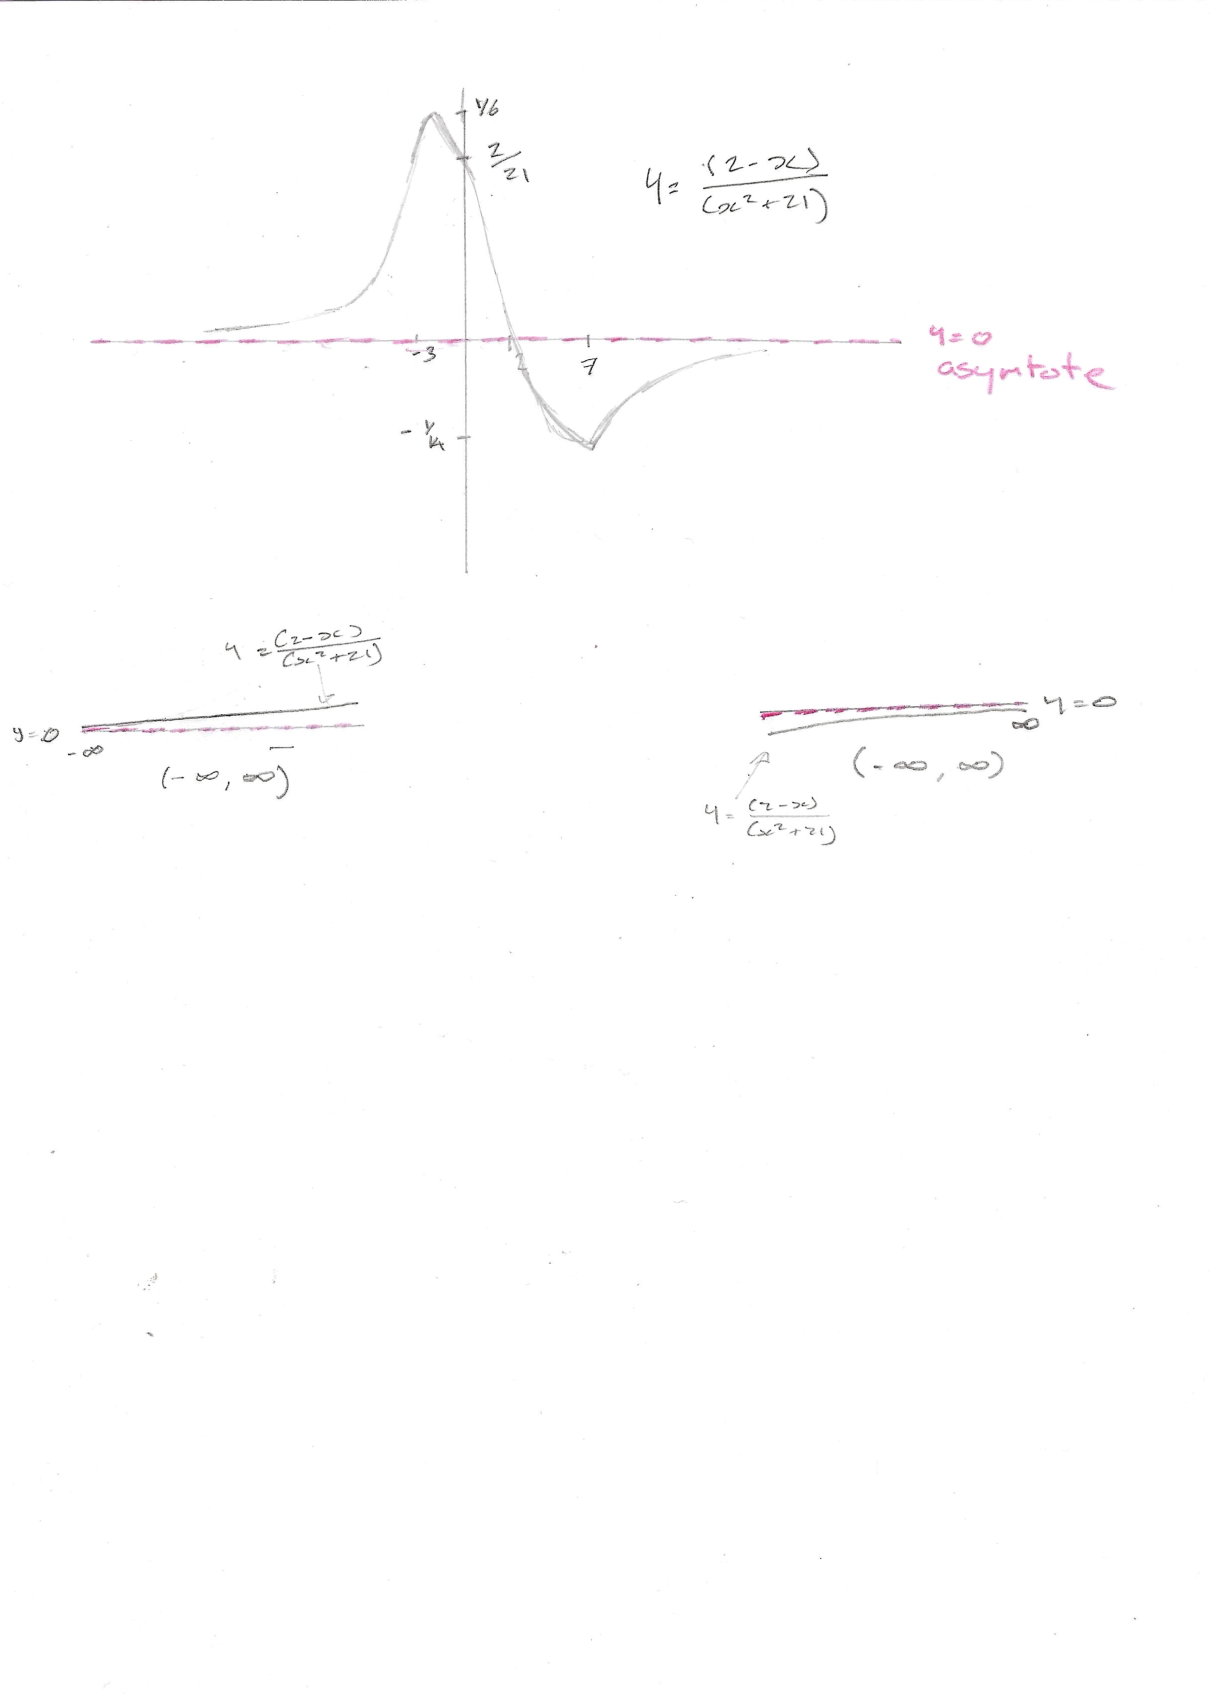
\includepdf[pages=-]{question_4_g.pdf}

\end{question}

\clearpage
%question five

\begin{question}

    \[ \int e^{x} \cosh^{3}(e^{x}) \dd{x} \]
    
\qpart

\marginnote{ \[ \cosh^{2}(x) = \frac{\cosh(2x) + 1}{2} \]}
\marginnote{ \[ cosh(x) = \frac{e^{x}+e^{-x}}{2} \]}
\marginnote{ \[ sinh(x) = \frac{e^{x}-e^{-x}}{2} \]}

Using the substitution \( u = e^{x} \), then \( du = e^{x} \dd{x} \).
\begin{align*}
    \int e^{x}\cosh^3(e^{x}) \dd{x} &= \int \cosh^3(u) \dd{u}\\[8pt]
   &= \int ( \cosh^{2}(u)\cosh(u) ) \dd(u)\\[8pt]
\stext{using half variable identiy}\\[8pt]
   &= \int  \frac{1}{2}( \cosh(2u) + 1 )\cosh(u) \dd{u}\\[8pt]
   &= \frac{1}{2} \int \cosh(2u)\cosh(u) \dd{u} + \frac{1}{2} \int \cosh(u) \dd{u}\\[8pt]
   &= \frac{1}{2} \int \frac{e^{-3u}}{4} \dd{u} + \frac{1}{2} \int \frac{e^{-u}}{4} \dd{u} 
   + \frac{1}{2} \int \frac{e^{u}}{4} \dd{u} + \frac{1}{2} \int \frac{e^{3u}}{4} \dd{u} 
   + \frac{1}{2} \int \cosh(u) \dd{u}\\[8pt]
   &= \frac{1}{8} \left( \int e^{-3u} \dd{u} + \int e^{-u} \dd{u} + \int e^{u} \dd{u} + \int e^{3u} \dd{u}  \right) + \frac{1}{2} \int \cosh(u) \dd{u}\\[8pt]
    &= \frac{1}{8} \left( -\frac{1}{3} e^{-3u} - e^{-u} + e^{u} + \frac{1}{3} e^{3u} \right) + \frac{1}{2} \sinh(u) + C\\[8pt]
    &= \frac{1}{8} \left( \frac{2}{3}sinh(3u) + 2\sinh(u)   \right) + \frac{1}{2} \sinh(u) + C\\[8pt]
    &= \frac{1}{12} \left( sinh(3u) + 9\sinh(u) \right) + C \\[8pt]
\stext{Substituting back for \( u = e^{x} \)}\\[8pt]
    &= \frac{1}{12} \left( sinh(3e^{x}) + 9\sinh(e^{x}) \right) + C\\[8pt]
\end{align*}

\vspace{5cm}

\qpart
\qsubpart

Using \( \cos{A}\cos{B} = \frac{1}{2}\cos(A+B)+ \frac{1}{2}\cos(A - B) \)

\begin{align*}
    \cos(2x)\cos(5x) &= \frac{1}{2}\cos(2x+5x) + \frac{1}{2}\cos(2x-5x)\\[8pt]
    &= \frac{1}{2}\cos(7x) + \frac{1}{2}\cos(-3x)\\[8pt]
\stext{Using the fact that \( \cos(-x) = \cos(x) \)}\\[8pt]
    &= \frac{1}{2}(\cos(7x) + \cos(3x))
\snote{As required}
\end{align*}

\vspace{3cm}

\qsubpart

    \[ \int \sin^{2}(x)\cos(5x) \]

\begin{align*}
\int \sin^{2}(x)\cos(5x) \dd{x} &= \int \frac{1}{2}(1 - \cos(2x))cos(5x) \dd{x}\\[8pt]
&= \frac{1}{2} \int cos(5x) \dd(x) - \frac{1}{2} \int \cos(2x)\cos(5x) \dd{x}\\[8pt]
\stext{Using the result from part (b)}\\[8pt]
&= \frac{1}{2} \int cos(5x) \dd{x} - \frac{1}{2} \int \left( \frac{1}{2}(\cos(7x) + \cos(3x)) \right) \dd{x}\\[8pt]
&= \frac{1}{2} \int cos(5x) \dd{x} - \frac{1}{4} \int \cos(7x) \dd{x} - \frac{1}{4} \int \cos(3x) \dd{x}\\[8pt]
&= \frac{1}{2} \times \frac{1}{5}\sin(5x) - \frac{1}{4} \times \frac{1}{7}\sin(7x) - \frac{1}{4} \times \frac{1}{3}\sin(3x) + C\\[8pt]
&= \frac{1}{10}\sin(5x) - \frac{1}{28}\sin(7x) - \frac{1}{12}\sin(3x) + C\\[8pt]
\end{align*}

\end{question}

\clearpage
%question six

\begin{question}

\qpart

\[ \dv{x}{t} = \frac{t^{7}}{(t^{8} + 32)^{\frac{3}{5}}} \]

This is a directly integrable first order differential equation. To solve it, 
we integrate both sides with respect to \( t \).

\qpart

\begin{align*}
    \int \dv{x}{t} \dd{t} &= \int \frac{t^{7}}{(t^{8} + 32)^{\frac{3}{5}}} \dd{t}\\[8pt]
    x(t) &= \int \frac{t^{7}}{(t^{8} + 32)^{\frac{3}{5}}} \dd{t}\\[8pt]
\stext{Using the substitution \( u = t^{8} + 32 \), then \( du = 8t^{7} \dd{t} \) }\\[8pt]
    &= \frac{1}{8} \int \frac{1}{u^{\frac{3}{5}}} \dd{u}\\[8pt]
    &= \frac{1}{8} \times \frac{u^{\frac{2}{5}}}{\frac{2}{5}} + C\\[8pt]
    &= \frac{5}{16} (t^{8} + 32)^{\frac{2}{5}} + C\\[8pt]
\end{align*}

\vspace{3cm}

\qpart

To find the particular solution that satisfies \( x(0) = 1 \).

\begin{align*}
    x(0) &= \frac{5}{16} (0^{8} + 32)^{\frac{2}{5}} + C\\[8pt]
    1 &= \frac{5}{16} (32)^{\frac{2}{5}} + C\\[8pt]
    &= \frac{5}{16} \times 4 + C\\[8pt]
    &= \frac{5}{4} + C\\[8pt]
    C &= 1 - \frac{5}{4}\\[8pt]
    &= -\frac{1}{4}\\[8pt]
\stext{Hence}
    x(t) &= \frac{5}{16} (t^{8} + 32)^{\frac{2}{5}} - \frac{1}{4}\\[8pt]
\end{align*}

\end{question}

\clearpage
%question seven

\begin{question}

    \[ \dv{y}{t} = \frac{\sqrt{1-y^{2}}}{t}, (t>0, -1<y<1) \]

\qpart
This is a separable differential equation. We can separate the variables and integrate both sides.

\vspace{3cm}

\qpart
\begin{align*}
    \int \frac{1}{\sqrt{1-y^{2}}} \dd{y} &= \int \frac{1}{t} \dd{t}\\[8pt]
    \sin^{-1}(y) &= \ln(t) + C\\[8pt]
\stext{Exponentiating both sides}\\[8pt]
    y &= \sin(\ln(t) + C)\\[8pt]
\end{align*}

\end{question}

\clearpage
%question eight

\begin{question}

    \[ x\dv{y}{x} - 4y = x^{5}sinh{x}, (x>0) \]

\qpart
This is a first order linear differential equation. We can rewrite it in standard form and find an
integrating factor.

\vspace{3cm}

\marginnote{The integrating factor is given by \[ p(x) = \exp\left( \int g(x) \dd{x} \right) \]}
\marginnote{The general solution for afirst order differential equation is 
\[ y = \frac{1}{p(x)}\left( \int p(x)h(x) \right) \]}

\qpart
\begin{align*}
    x\dv{y}{x} - 4y &= x^{5}sinh(x)
\stext{Divide by \( x \)}\\[8pt]
    \dv{y}{x} - \frac{4}{x}y &= x^{4}sinh(x)\\[8pt]
\stext{This is in the form \( \dv{y}{x} + g(x)y = h(x) \)}\\[8pt]
\stext{Where}
    p(x) &= \exp\left( \int \frac{4}{x} \dd{x} \right)\\[8pt]
    &= \exp(4\ln(x))\\[8pt]
    &= x^{4}\\[8pt]
\stext{Using this to write the general solution}
    y &= \frac{1}{x^{-4}}\left( \int x^{-4}(x^4\sinh(x)) \dd{x} \right)
    &= x^{4}\left( \int \sinh(x) \dd{x} \right)\\[8pt]
\stext{Integrating \( \sinh(x) \)}\\[8pt]
    &= x^{4}(\cosh(x) + C)\\[8pt]
\end{align*}

\end{question}

\clearpage
%question nine

\begin{question}

    \[ \dv{y}{t} = \frac{1}{10000}(100 - y)  \text{Where} y(0)=30\]

\qpart
This is a first order linear differential equation. We can separate the variables and integrate both sides.
 
\begin{align*}
    \int \frac{1}{100 - y} \dd{y} &= \int \frac{1}{10000} \dd{t}\\[8pt]
\stext{Let \(  u=100-y \) and \( du = -\dd{y} \)}\\[8pt]
    -\int \frac{1}{u} \dd{u} &= \frac{1}{10000} \int \dd{t}\\[8pt]
    -\ln|u| &= \frac{t}{10000} + C\\[8pt]
\stext{Substituting back for \( u = 100 - y \)}\\[8pt]
    -\ln(100 - y) &= \frac{t}{10000} + C\\[8pt]
\stext{Exponentiating both sides}\\[8pt]
    100 - y &= e^{-\frac{t}{10000} - C}\\
    100 - y &= {A}e^{-\frac{t}{10000}} 
    \snote{ where  \( A = e^{-C} \) }\\[8pt]
\stext{Rearranging gives us the general solution}\\[8pt]
    y &= 100 - Ae^{-\frac{t}{10000}}\\[8pt]
\end{align*}

\vspace{5cm}

\qpart
To find the particular solution that satisfies \( y(0) = 30 \).

\begin{align*}
    y(0) &= 100 - Ae^{-\frac{0}{10000}}\\[8pt]
    30 &= 100 - A\\[8pt]
    A &= 70\\[8pt]
\stext{So the particular solution is}
    y &= 100 - 70e^{-\frac{t}{10000}}\\[8pt]
\stext{This can be simplified to}
    y &= 100 - 70e^{-\frac{t}{10000}}\\
\end{align*}

\vspace{3cm}

\qpart

After \( \SI{600}{\second} \);

\begin{align*}
    y(600) &= 100 - 70e^{-\frac{600}{10000}}\\[8pt]
    &= 100 - 70e^{-\frac{3}{50}}\\[8pt]
    &= 100 - 70 \times e^{-0.06}\\[8pt]
    &= 100 - 70 \times 0.9417\ldots\\[8pt]
    &= 100 - 65.9235\ldots\\[8pt]
    &= 34.0764\ldots\\[8pt]
    &= \SI{34}{\kilo\gram}\\[8pt]
\snote{To 2 s.f}
\end{align*}

\vspace{3cm}

\qpart

As \( t \to \infty \), the term \( e^{-\frac{t}{10000}} \) approaches zero, so
\begin{align*}
    y(t) &\to 100 - 70 \times 0\\[8pt]
    &= 100\\[8pt]
\stext{So the limiting value of \( y \) as \( t \to \infty \) is \( \SI{100}{\kilo\gram} \).}  
\end{align*}

\vspace{3cm}

\qpart

\subsection*{Question 9 (e)}
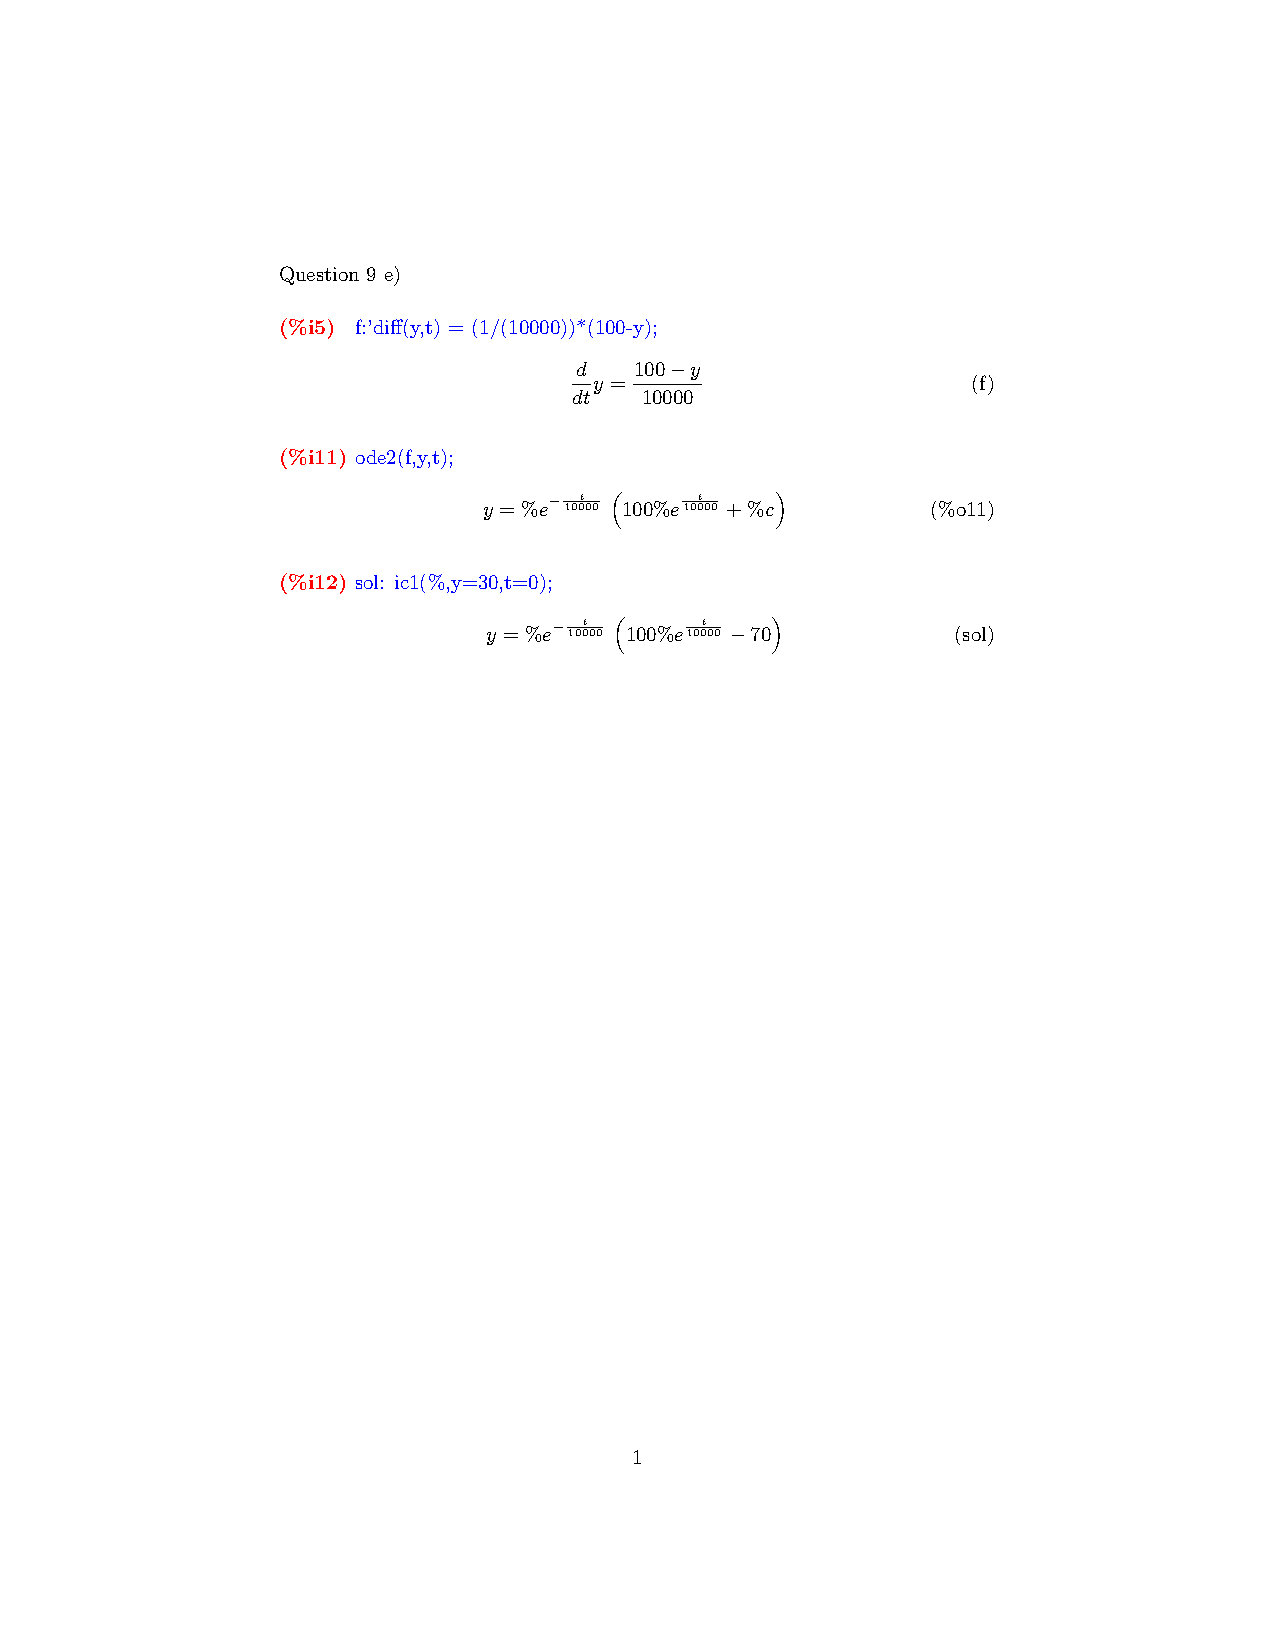
\includepdf[pages=-]{question_10_e.pdf}

\end{question}

\clearpage
%question ten
\begin{question}

\end{question}
\clearpage

\end{document}